\subsection{Tonhöhen- und Lautstärkenoszillator}\label{subsec:Antennenoszilator}
Für die Antennenoszillator-Schaltung haben wir uns im Projekt 5 für den Colpitts-Oszillator aus Abbildung \ref{img:colpitts} entschieden. Der Aufbau im Projekt 5 umfasste nur einen Oszillator zur Veränderung der Tonhöhe.

Es handelt sich dabei um einen Colpitts-Oszillator mit einem JFET. Diese Schaltung ist von dem Bauset ''Theremin selber bauen`` von Franzis übernommen \cite{Franzis}. 
Da der im Bauset verwendete JFET nicht mehr bestellbar ist, war ein Wechsel auf den J113 N-Kanal JFET nötig. Die mit LTspice simulierten Werte des J113 glichen stark der Originalschaltung, weshalb der Entscheid auf diesen fiel. 
Damit das Sinussignal des Antennenoszillator nicht A/D gewandelt werden muss, wandelt eine Komparatorschaltung das Sinussignal in ein Rechtecksignal mit gleicher Frequnez um. 
Diese ist mit \SI{3.3}{V} betrieben, da die Logikeingänge des FPGA auf diese Spannung ausgelegt sind. 

Im Projekt 5 wurde als Antenne ein Messingrohr verwendet. Diese ist am Anschluss pitch\_antenna verbunden. 

Die Ausgangsspannung des Colpitts-Oszillator ist über den Kondensator C11 entkoppelt. Dies entfernt den DC-Anteil. Der Kondensator C11 und die Widerstände R3 und R4 bilden zusammen einen Hochpass. Damit die Oszillatorfrequenz von ca \SI{562}{kHz} das Filter passieren kann, ist C11 so gewählt, dass die Grenzfrequenz des Filters bei ca \SI{265}{kHz} liegt. 

Auf dem PCB sind nun im Projekt 6 zwei solche Oszillatoren verbaut: Der Tonhöhenoszillator und der Lautstärkenoszillator. Das PCB ist mit einem \SI{12} {VDC} Schaltnetzteil gespiessen. Der MC7809 Spannungsregler generiert die \SI{9} {VDC} für die Colpitts-Oszillatorschaltungen. Die \SI{3.3} {VDC} für den Komperator erzeugt der LT1117 Spannungsregler. Bei der Wahl der Spannungsregler ist darauf geachtet worden, dass die erzeugten Spannungen möglichst störungsfrei ist und wenig Ripple aufwiesen. Das gesamte Schema der Schaltung ist im Anhang enthalten.

\begin{figure}[h]
	\centering
	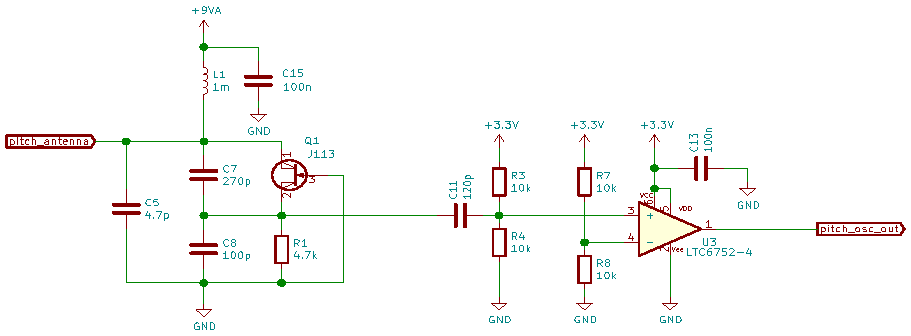
\includegraphics[width=\textwidth]{colpitts.pdf}
	\caption{Schema Antennenoszillator. Links Collpitts-Oszillator, rechts Komparatorschaltung}
	\label{img:colpitts}
\end{figure} 

\clearpage


